\documentclass{article}
\usepackage{chemformula}
\usepackage{import}
\usepackage[utf8]{inputenc}
\usepackage{float}
\usepackage{graphicx}
\usepackage{tikz}
\usepackage{amsmath}
\usepackage{tikz}
\pagestyle{empty}
\usepackage{vmargin}
\usepackage{newtxtext}
\usepackage{relsize}
\usepackage{wrapfig}
\usepackage{lipsum}
\usepackage{blindtext}
\usepackage{caption}
\usepackage{pdflscape}
\captionsetup{labelfont=bf}
\renewcommand{\figurename}{\textbf{Imagen}}


%%Peio Lopez, Ander Gorocica, Sergio Lusa \\ Unai Bermudez, Mikel Goti


\begin{document}

\begin{titlepage}
   \begin{center}
    \textsc{\LARGE{Gestión de Naviera Marítima}}\\
        \vspace*{2.6cm}
        \secondtitle{Grado en Ingeniería Informática de Gestión y Sistemas de Información}
        \line(1,0){400}
        \vspace*{0,8cm}\\
        
         \huge{\bfseries ENTREGA FINAL\\
         \vspace*{0,55cm}
         \line(1,0){360}

       \vspace{3cm}
            \textsc{\LARGE{Diseño de Bases de Datos}}\\
        \vspace{1.5cm}
            \begin{logo}
                
\includegraphics[width=.99\textwidth]{img/UPV.jpg}
            \end{logo}
    \end{center}
        \vspace{1.2cm}
        \begin{flushright}
        \begin{logo}
            
\includegraphics[width=2.5cm, height=1.5cm]{img/logo.png}
        \end{logo}\\
        \vspace{0.3cm}
        \textsc{
        Peio Lopez, Ander Gorocica, Sergio Lusa \\ Unai Bermudez, Mikel Goti\\
        }\\
        \vspace{0.3cm}
                    08/12/2023
            
        \end{flushright}
\end{titlepage}

\newpage
\tableofcontents
\newpage

\section{Introducción}

En este informe, se presenta la descripción de la funcionalidad que se desea implementar para una naviera que transporta tanto pasajeros como mercancías, así como la propuesta de una expansión o módulo adicional que se podría añadir al juego existente. Este proyecto tiene como objetivo diseñar una base de datos que respalde las operaciones de esta naviera y permita una gestión eficiente de sus recursos y servicios.

\section{Descripción Básica (Hito 1)}

La naviera en cuestión se dedica al transporte de pasajeros y mercancías a través de rutas marítimas. Para ello, necesita una plataforma de gestión que le permita registrar y controlar los siguientes aspectos:

\begin{itemize}
    \item Información de los barcos utilizados, incluyendo numero identificador, nombre, dimensiones, año de fabricación, etc. A parte de estos atributos también distinguiremos los barcos según su tipo, los destinados a trasporte de mercancías y los destinados a transporte de pasajeros. En los barcos destinados a transporte de mercancías tendremos atributos como capacidad de carga y numero de contenedores. Y en los barcos destinados a transporte de pasajeros tendremos atributos como capacidad de pasajeros y numero de camarotes.
    \item Registro de rutas marítimas, con detalles sobre los puertos de origen y destino, horarios de salida/llegada, código identificador de la ruta, longitud del trayecto, tarifas, etc. Cada barco tendrá asociadas una o varias rutas marítimas que pueda realizar
    \item Registro de pasajeros de nuestro sistema en el que almacenaremos datos personales como DNI, nombre, apellidos, teléfono, Email, fecha de nacimiento, etc.
    \item Reservas realizadas en una de nuestras rutas. De estas reservas se almacenará un id único para cada reserva, el DNI de la persona que ha realiza la reserva, la ruta reservada y el horario de la misma.
    \item Gestión de Tripulación: Este módulo permitirá a la naviera administrar la información relacionada con la tripulación de sus barcos. Incluirá campos para registrar el nombre de los miembros de la tripulación, sus roles (capitán, marinero, chef, etc.), fechas de contratación y terminación de contratos, y certificaciones requeridas (por ejemplo, licencias de navegación).
    \item Programación de Horarios de la Tripulación: Este módulo permitirá a la naviera programar los horarios de trabajo de la tripulación. Los usuarios podrán asignar miembros de la tripulación a rutas específicas en días y horarios determinados. También podrán gestionar las ausencias y permisos de la tripulación.
\end{itemize}\\

\section{Conclusión}\\

Hasta el momento, hemos definido la funcionalidad principal de nuestro proyecto, que es proporcionar una base de datos sólida para la naviera que transporta pasajeros y mercancías por rutas marítimas. Hemos identificado la necesidad de gestionar información detallada sobre barcos, rutas marítimas, pasajeros y reservas. Además, hemos propuesto un módulo adicional centrado en la Gestión de Tripulación, que permitirá una administración eficiente de los miembros de la tripulación y la programación de horarios. Este enfoque garantizará una gestión efectiva de los recursos y servicios de la naviera

\begin{landscape}
\section{Diseño conceptual de la BD (Hito 2)}
\begin{figure}[H]
    \begin{center}
    \end{center}
    \centering
    \vspace{0.3cm}
    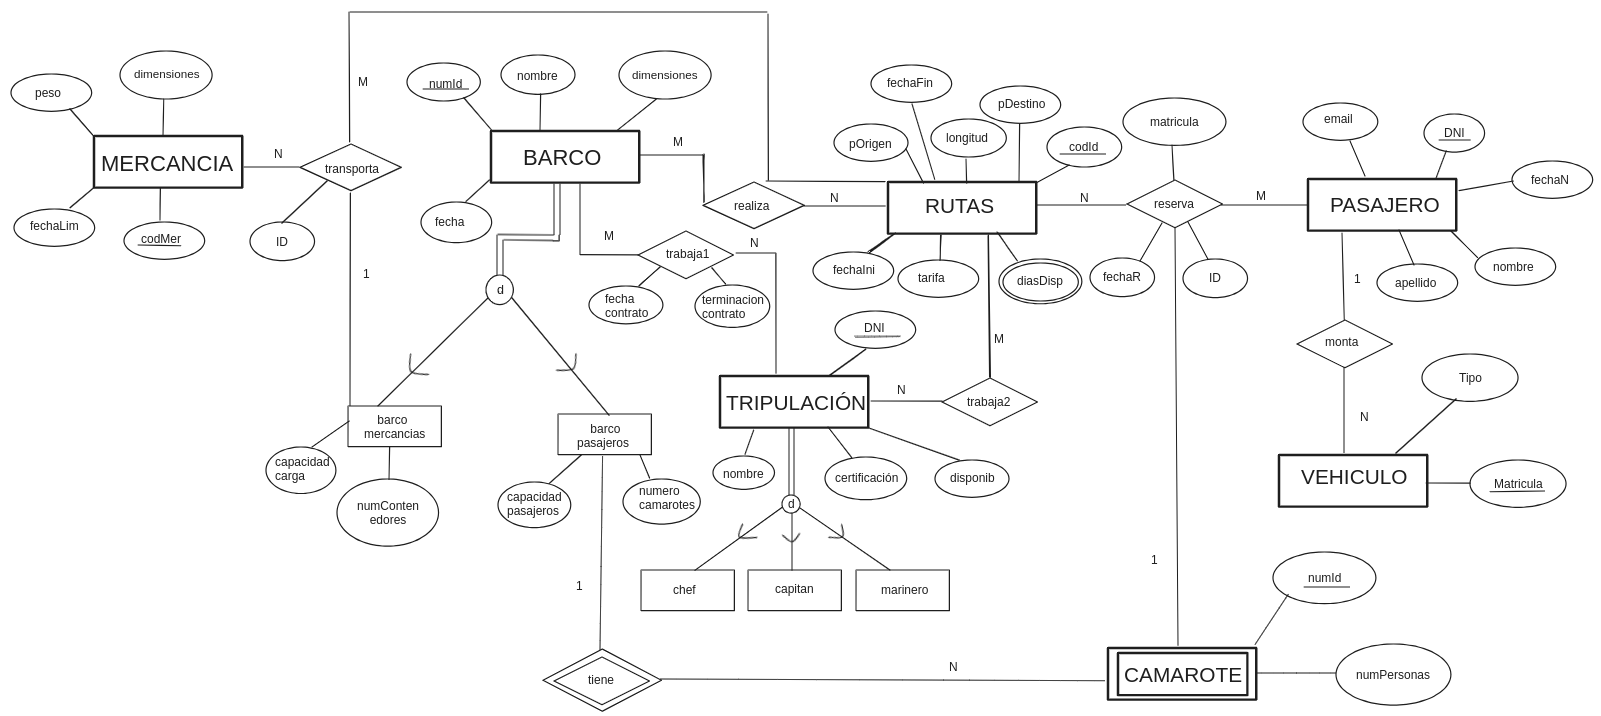
\includegraphics[width=600pt, angle=0]{img/DBD_esquemaBD.png}
    \caption{Diagrama de Esquema Relacional de la Base de Datos}
    \vspace{0.3cm}
    \label{titulua}
\end{figure}
\end{landscape}


\section{Tercera parte}
\subsection{Tablas de la base de datos}


BARCO (\underline{numID}, nombre, dimensiones, fecha)\\\\
BARCO-MERCANCIAS (\underline{numID}, cantCarga, nContenedores)\\\\
BARCO-PASAJEROS (\underline{numID}, cantPasajeros, nCamarotes)\\\\
TRIPULACION (\underline{DNI}, nombre, certificación, disponib)\\\\
CHEF (\underline{DNI})\\\\
CAPITAN (\underline{DNI})\\\\
MARINERO (\underline{DNI})\\\\
MERCANCIA (\underline{codMerc}, peso, fechaLim, dimendiones)\\\\
RUTAS (\underline{codID}, pOrigen, pDestino, fechaIni, fechaFin, longitud, tarifa)\\\\
PASAJERO (\underline{DNI}, nombre, apellido, email, fechaN)\\\\
VEHICULO (\underline{matricula}, tipo, DNIDueno)\\\\
CAMAROTE (\underline{numId}, \underline{numIdBarco}, nPersonas)\\\\
REALIZA (\underline{nomIDBarco}, \underline{codIDRuta})\\\\
TRABAJA1 (\underline{nomIDBarco}, \underline{DNITripulante}, fechaContrato, terminacionContrato)\\\\
TRABAJA2 (\underline{codIDRuta}, \underline{DNITripulante})\\\\
DIASDISPONIBLES (\underline{codID}, \underline{diaDisp})\\\\
TRANSPORTA (\underline{codMerc}, \underline{codIDRuta}, \underline{nomIDBarco}, id)\\\\
RESERVA (\underline{codIDRuta}, \underline{DNIPasajero}, \underline{numIDCamarote}, \underline{numIDBarco}, matricula, fechar, ID)\\\\


\newpage
\subsection{Modificación del diseño para mejorar la búsqueda}
No vamos ha cambiar nada porque nuestro diseño es conveniente para realizar esta búsqueda.\\\\
Para calcular los viajes que ha realizado cada trabajador este ultimo año, por cada trabajador tendremos que hacer una consulta en la tabla TRABAJA2 que almacena la relación entre la tabla Trabajador y la tabla Ruta, para cada trabajador haremos una consulta en esta tabla que haga coincidir el DNI y la fechaInicio y la fechaFin de la ruta coincidan con la fecha del año actual. \\\\
Luego realizaremos un count de todas las tuplas que existen en esta tabla para saber cuantos viajes a realizado. Finalmente utilizaremos DATEDIFF ( day , fechaInicio , fechaFin ) para calcular la duración de la ruta, y sumaremos la duración de todas las rutas para saber cuantos días ha trabajado en total cada tripulante. \\\\
Aún así, para no tener que calcular la diferencia de días constantemente cada vez que queremos buscar cuantos días ha trabajado cada tripulante se podría introducir en cada ruta la duración de la ruta (en días). 
\clearpage
\subsection{Solución para la nueva funcionalidad}

\vspace{0.5cm}

Cuando un cliente realiza una transacción, se registra en la tabla Transacciones.\\

Un proceso automático o un disparador (trigger) en la base de datos podría calcular los puntos acumulados y actualizar la tabla Puntos en función de las transacciones realizadas.\\

Cuando un cliente desea utilizar sus puntos para obtener un descuento, se registra en la tabla Descuentos, y el monto del descuento se descuenta del total en la transacción actual.\\

Puedes consultar fácilmente el historial de transacciones, puntos acumulados y descuentos para un cliente específico mediante las relaciones establecidas.\\

\vspace{0.5cm}

\begin{logo}
    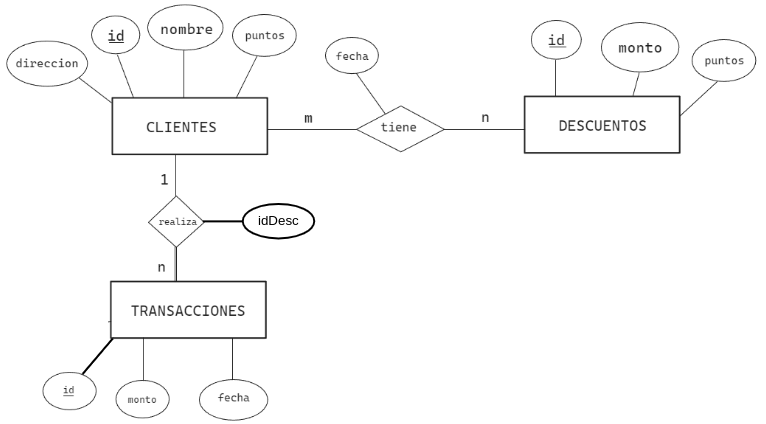
\includegraphics[width=.99\textwidth]{img/db.png}
\end{logo}

La tabla \textbf{clientes} almacenará la información básica del cliente de la pagina web, como el ID del cliente, nombre, dirección. El ID será necesario como clave primaria para poder identificar al cliente y registrar sus transacciones.\\


\clearpage


\subsection{Necesidades de mejora e índices}
Los índices se utilizan para estructurar datos y consecuentemente acelerar la obtención de registros para búsquedas concretas. En nuestro caso, observando el esquema relacional de nuestra base de datos se pueden identificar dos necesidades de mejora, en las que sería recomendable utilizar índices. La parte central de nuestro esquema relacional serían las rutas, ya que, tiene vínculos con la mayor parte de entidades, por lo tanto, los dos índices que se han planteado están relacionados con esa tabla. 
\newline
\newline
Una de ellas podría ser utilizar un índice en la tabla "TRABAJA2" para buscar de manera más eficiente que rutas realiza cada tripulante y de esta manera se podría obtener de una manera más sencilla información relevante, como, la cantidad de días que trabaja un trabajador anualmente. 
\newline
\newline
Para ello se generaría el siguiente índice principal, ordenado por la clave primaria de la tabla y agrupado por bloques, ya que, se supone que se van a realizar muchas rutas.
\begin{verbatim}
CREATE INDEX idx_tripulante_ruta ON TRABAJA2 (DNITripulante, codIDRuta);
\end{verbatim}
Otra de las necesidades de mejora son las reservas, dado que van a ser una de las consultas más usadas en la naviera y se quieren realizar de manera rápida para que los pasajeros estén esperando el menor tiempo posible.
\newline
\newline
Para gestionar las reservas se generaría un índice con el que se puedan realizar búsquedas de las fechas de las rutas y el número de pasajeros que caben en el camarote.
\begin{verbatim}
    CREATE INDEX idx_reservas_rutas ON 
    RESERVA (codIDRuta, numIDCamarote), 
    RUTAS (codID, fechaIni, fechaFin),
    CAMAROTE (numId, nPersonas);
\end{verbatim}
\clearpage

\subsection{Restricciones de integridad}

Las aserciones (assertions) se utilizan para especificar condiciones que deben ser siempre verdaderas en la base de datos, mientras que los triggers (disparadores) son bloques de código que se ejecutan en respuesta a ciertos eventos, como la inserción, actualización o eliminación de datos.\\

La principal diferencia es que las aserciones son evaluadas globalmente en la base de datos, independientemente de las operaciones que se estén realizando, mientras que los triggers responden a eventos específicos.

\subsubsection{TRIGGER}

Una forma de introducir un \textbf{trigger} en el proyecto podría ser en la nueva funcionalidad de la pagina web, a la hora de cualcular los descuentos según los puntos.\\

Para mantener las ofertas actualizadas y proporcionar los descuentos según las transacciones del cliente se podría definir un \textbf{trigger} para calcular los puntos por cada transacción. De esta forma los puntos que tiene cada cliente se calcularián a partir de cada transacción automaticamente.\\

Este procedimiento almacenado está diseñado para calcular los puntos acumulados para un cliente específico en función del monto de una transacción y actualizar la tabla Puntos.

\begin{verbatim}
CREATE PROCEDURE CalcularPuntos(IN p_TransaccionID INT)
BEGIN
    -- Declaración de variables locales
    DECLARE v_Monto DECIMAL(10, 2);
    DECLARE v_PuntosAcumulados INT;

    -- Obtener el monto de la transacción
    SELECT Monto INTO v_Monto FROM Transacciones WHERE TransaccionID = p_TransaccionID;

    -- Calcular los puntos (1 punto por cada euro gastado)
    SET v_PuntosAcumulados = ROUND(v_Monto);

    -- Actualizar la tabla Puntos
    UPDATE Puntos SET PuntosAcumulados = PuntosAcumulados + v_PuntosAcumulados
    WHERE ClienteID = (SELECT ClienteID FROM Transacciones WHERE TransaccionID = p_TransaccionID);

DELIMITER ;
\end{verbatim}

\subsubsection{ASSERTION}

Una posible implementación de una \textbf{aserción} en la base de datos podría ser que la suma total de la cantidad de carga (cantCarga) en los barcos de mercancías no exceda cierto límite global.

\begin{verbatim}
    CREATE ASSERTION LimiteCargaGlobal
    CHECK (
    (SELECT SUM(peso) FROM MERCANCIAS) <= 10000);
\end{verbatim}

De está forma nos aseguramos de que la suma de la carga de cada barco no exceda los 10000 kg.


\end{document}
